%!TEX root = ../main.tex

\newcommand{\Titel}{Risikoanalyse}
%!TEX root = ../main.tex

\begin{titlepage}
	\begin{center}
		\vspace*{-2.5cm}
		\hfill	
\includegraphics[width=5cm]{images/dhbw.png}\\[5cm]
		
		{\Huge \scshape \Titel}\\[1cm]
		{\large für die Erstellung der Studienarbeit}\\[0.5cm]
		\vspace{1cm}
		
		%{\large von}\\[0.5cm]
		%{\large \Autor \ \& \AutorZwei}\\[1cm]
		
		\vfill
	\end{center}
	\begin{tabular}{l@{\hspace{2cm}}l}
		\bfseries Teilnehmer & \Teilnehmer      \\
		\bfseries Datum      & \DatumUndZeit      \\
		\bfseries Ort        & \Ort             \\
		\bfseries Thema      & \Thema           \\
		\bfseries Betreuer   & \Betreuer        \\
		\bfseries Kurs       & \Kursbezeichnung
	\end{tabular}
	
\end{titlepage}


\section{Risikobetrachtung}
In der nachfolgenden Tabelle sind einige möglichen Risiken abgebildet.
Sie sind nach Risikofaktor sortiert, der sich mit der Formel $Wahrscheinlichkeit * Schwere * 10$ berechnet.

\begin{center}
	\makebox[\textwidth]{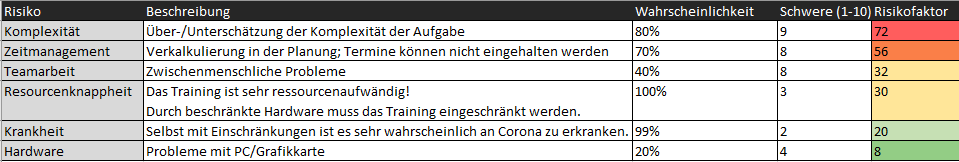
\includegraphics[width=1.0\textwidth]{allgemein/risiko/Risiken.png}}
\end{center}

\section{Gegenmaßnahmen}
In der nachfolgenden Tabelle sind Gegenmaßnahmen zu den zuvor identifizierten Risiken aufgelistet.
Verantwortlich für die Beachtung der Risiken und Gegenmaßnahmen sind dabei alle Teammitglieder.
Dadurch ist eine zusätzliche gegenseitige Kontrolle gewährleistet.

\begin{center}
	\makebox[\textwidth]{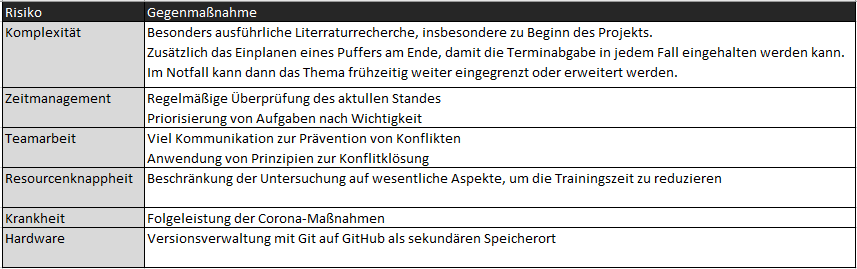
\includegraphics[width=1.0\textwidth]{allgemein/risiko/Gegenmassnahmen.png}}
\end{center}
